%!TEX root = karen.tex

\chapter{Stokes (Incomplete)}

This whole chapter is incomplete work. We started working toward stoke solutions on the unit sphere but it has yet to be completed. 

\section{Introduction}

We consider herein the solution to steady-state viscous Stokes flow on the surface of a sphere, governed by: 
%TODO: 	\authnote{Where did we go wrong? Our vector laplacian does not have a curl component included. How do we derive that from here?} 
% We actually went wrong because $u$ is a vector. That means that the $\grad$ operator is actually a Jacobian matrix.
% We also f-d up \div ( n F) = \grad n dot F + n \div F. (i.e., the term cannot be moved out easily). Really unless we rederive
% from scratch this whole section amounts to: a mock system of coupled scalar PDEs. 
  \begin{align}
\div{[\eta(\grad{\vu} + (\grad{\vu})^T)]} + Ra T \hat{r} & = \grad{p} \label{eq:stokes_momentum} \\
%\pd{T}{t} + (\vu \cdot \grad) T & = \Laplacian T \ \ \ \ \ \ \ \ \textsl{(Energy)}\label{eq:stokes_energy}
\div{\vu} & = 0 \label{eq:stokes_continuity} 
\end{align}
where the unknowns $\vu$ and $p$ represent the vector velocity- and scalar pressure-field respectively, $\eta$ is the viscosity tensor, $Ra$ is the non-dimensional Rayleigh number, and $T$ is an initial temperature profile. Many practical applications in sciences such as geophysics, climate modeling, and computational fluid dynamics must solve variations of the Navier-Stokes equations. The focus of this paper is on the implicit solve component for viscous (Stokes) flow, which amounts to the steady-state problem described by Equations~\ref{eq:stokes_momentum} and \ref{eq:stokes_continuity}. 



This article introduces the first (to our knowledge) parallel approach to solve the steady-state equations on the surface of the unit sphere with the Radial Basis Function-generated Finite Differences (RBF-FD) method. Building on our work in \cite{BolligFlyerErlebacher2012}, which parallelized explicit RBF-FD advection, our goal is to integrate both explicit and implicit components within a larger transient flow model. 


For decades, the demand for fast and accurate numerical solutions in fluid flow has lead to a plethora of computational methods for various geometries, discretizations and dimensions.  On the sphere in $\R^3$ popular discretizations include the standard latitude-longitude grid, cubed-sphere \cite{NairTransport05}, yin-yang overlapping grid \cite{Kameyama2008a}, icosahedral grid \cite{Randall2002} and centroidal voronoi tessellations \cite{Du2006}. Associate with each discretization is a mesh---specific to the choice of numerical method---that indicates connectivity of nodes for differentiation.


Until now, most of the focus in RBF-FD has been on explicit methods. However, many practical applications in sciences such as geophysics, climate modeling, and computational fluid dynamics must solve variations of the Navier-Stokes equations, and depend on an implicit solve component. This paper develops multi-GPU algorithms for implicit RBF-FD systems toward the goal of integration within transient flow problems. %The explicit component of transient flow is a natural extension of our work in \cite{BolligFlyerErlebacher2012}. 

%TODO: Speed not the issue. Functioning solutions first. 
%TODO: Need less RBFs for given accuracy of steady state
%TODO: less nodes implies less memory
%TODO: general geometries are supported
%TODO: better distributions of nodes on spheres. competition like CitComS, etc. use cubed sphere, yinyang grids and triangular meshes in combination with low order methods (2nd and 3rd order). Increasing the order of the method or dimension can significantly increase the complexity of the algorithms. RBF-FD naturally extends to higher dimensions and increasing the order is as simple as increasing the number of nodes in the stencil. 

%TODO: Related work
%TODO: divergence-free spherical radial basis Glerkin method for Stokes on the unit sphere \cite{Ganesh2011} 
%TODO: Incompressible Navier-Stokes using explicit (Euler) and semi-implicit (Crank Nicholson) time step. Small problem size  ($61 x 61$) and small stencil sizes ($n=9$); ghost nodes beyond boundary strategy.  Both RBF-FD and RBF-HFD tested. \cite{Chinchapatnam2009}
%TODO: Related work on Preconditioned iterative methods for Stokes Flow
%\begin{itemize}
%\item Survey of preconditioners used for Stokes flow problems \cite{May2008} (limited applicability since they do not assume non-SPD matrices) 
%\item Multi-GPU Jacobi iteration for Navier stokes flow in cavity \url{http://scholarworks.boisestate.edu/cgi/viewcontent.cgi?article=1003&context=mecheng_facpubs}
%\end{itemize} 

Our goal is to demonstrate to the geosciences that RBF-FD can function well on
both hyperbolic and elliptic problems. In \cite{BolligFlyerErlebacher2012} we
introduced a multi-GPU implementation of RBF-FD and demonstrated the method's
strong ability to stably advect solid bodies on the sphere. In this paper we
continue toward the goal of RBF-FD solutions for fluid flow problems with a
multi-GPU Poisson solver for steady-state Stokes flow. In this context, speed is
not a paramount issue.

Related work on RBF methods targeting the GPU is quite limited. Schmidt et al.
\cite{Schmidt2009b} solve an implicit system for a global RBF method using
Accelerys Jacket in Matlab. Our work in \cite{BolligFlyerErlebacher2012} introduced the first
parallel implementation of RBF-FD for explicit advection capable of spanning
multiple CPUs as well as multiple GPUs. 

Related work on multi-CPU or multi-GPU RBFs
\begin{itemize} 
	\item CPU \cite{Yokota2010} \cite{Wildemann2009}
	\item single-GPU \cite{Schmidt2009b}
	\item multi-GPU 
	\begin{itemize} 
	\item Preconditioned BiCGStab for Navier Stokes, Finite Element method \cite{Goeddeke2009a} 
	\end{itemize} 
\end{itemize} 

While RBF-FD differentiation matrices are applied in the same fashion as standard FD methods, they are unique in that they are asymmetric, non-positive definite and potentially have high condition numbers. To solve an implicit system therefore, we requie an iterative krylov solver like GMRES or BiCGStab which are applicable to matrices of this type. Additionally, preconditioned variants of these methods are required to reduce the complexity of the solution process. 

Within this paper we implement a preconditioned GMRES method for RBF-FD on multiple GPUs. 

Parallel GMRES
\begin{itemize} 
	\item CPU only: PETSc \cite{Yokota2010}, Hypre \cite{Wildemann2009} 
	\item Parallel GMRES on single GPU available in ViennaCL \cite{Rupp2010} and CUSP \cite{Cusp2012}
	\item Parallel GMRES on Multiple GPUs \cite{Bahi2011}
	\item Reduced Communication with increased computation \cite{Dekker2000}
\end{itemize} 

This article continues our effort with an implementation of RBF-FD on both single and multiple-GPUs for elliptic PDEs. In the next section we introduce 

%\section{Bad Problem} 
%
%Our initial derivation of the Stokes problem was incorrect. What we thought was
%the proper identity reduced the problem to simple scalar velocity laplacians and
%pressure gradients. The correct formulation of Stokes flow in 3D would have a
%curl component connecting each dimension. 
%
%Rather than start over and reformulate our problem, we opted to continue
%development of our GPU-based solver with the recognition that the problem we
%posed is actually a coupled Poisson problem and can be solved using the same
%iterative solver. By implementing and testing the solver and preconditioners for
%one problem, we prepare for the other.  
%
%\subsection{Details}
%Items to test for our solver: GFLOPs throughput (CPU,GPU), Convergence of Solver (in
%iteration residual) vs Preconditioners.
%
%Test problems: Sphere coupled poisson. Annulus. Stokes on annulus? 
%
%

\section{Multi-GPU GMRES}

Our implementation leverages ViennaCL to directly benefit from improvements to the performance of underlying sparse matrix-vector product, vector dot vector and other linear algebra primitives. Also, ViennaCL provides seamless interoperability with the Boost::UBLAS, EIGEN and MTL libraries via C++ templates. We test the performance of our algorithm on one or more CPUs with the Boost::UBLAS library. 

%TODO: Table comparing CUSP and ViennaCL features in GPU SpMV chapter?

The GMRES algorithm was introduced in 1986 by Saad and Schultz \cite{Saad1986}. The iterative solver support general matrix structures, whereas methods like Conjugate Gradient require symmetric positive definiteness. 


At the core of the GMRES algorithm is an Arnoldi (orthogonalization) process. %TODO: \authnote{significance of orthogonalization}. 

%TODO: variants in orthogonalization steps and variants in preconditioners, actual iterations, restarts etc. 
Variants of GMRES exist that utilize unique orthogonalization steps. The motivation behind alternative Arnoldi processes is to save both memory and operation counts. %In some cases stability of the GMRES iterations can also be improved \cite{FindRef}. 
Saad \cite{Saad1986} introduced a practical implementation of the GMRES method based on Given's rotations to compute an implicit QR factorization. The Given's based algorithm is part of libraries like CUSP \cite{Cusp2012} and CULA Sparse \cite{CULA}; ViennaCL implements the Householder reflection algorithm. 

The Given's rotation algorithm is easier to parallelize than Householder, which led to the addition of an alternate GMRES algorithm with restarts under ViennaCL. 

The authors of \cite{Bahi2011} do not describe their orthogonalization process, but based on the description of their parallelization strategy it is safe to assume a Given's rotation is used.

Algorithm~\ref{alg:gmres} presents the basic Left-preconditioned GMRES algorithm with restarts and Given's rotations. The comments in blue denote portions of the algorithm that depend on MPI collectives and the MPI routine used . 


%TODO: The Arnoldi process can be completed using in a variety of ways. Some libraries like CUSP and \cite{Saad2003} prefer the straightforward Givens rotations because they are easily parallelizable. The givens algorithm is provided in Algorithm~\ref{alg:gmres_givens}

%TODO: Others like [...] prefer to use an alternate algorithm. This algorithm is demonstrated in Algorithm~\ref{alg:gmres_h}.


\begin{algorithm}                      % enter the algorithm environment
\caption{Left-preconditioned GMRES(k) with Given's Rotations}          % give the algorithm a caption
\label{alg:gmres}                           % and a label for \ref{} commands later in the document
\begin{algorithmic}[1]                    % enter the algorithmic environment
    \State $\varepsilon$ (tolerance for the residual norm $r$), $x_0$ (initial guess), and set $convergence = false$
   	\State {\color{blue} MPI\_Alltoallv($x_0$)}
    \While{ $convergence == false$}  
    \State $r_0 = M^{-1} (b-Ax_0)$
   	\State {\color{blue} MPI\_Alltoallv($r_0$)}
    \State $\beta = ||r_0||_2$			\Comment{{\color{blue} MPI\_Allreduce($<r_0,r_0>$)}}
    \State $v_1 = r_0 / \beta$ 

	\For {$j=1$ to $k$} \label{alg:gmres_rotation_loop_start} 
			\State $w_j = M^{-1} A v_j$   
			\Comment{{\color{blue} MPI\_Alltoallv($w_j$)}}
			\For {$i = 1$ to $j$}\label{alg:gmres_inner_loop_start}
				\State $h_{i,j} = <w_j, v_i>$ \Comment{{\color{blue} MPI\_Allreduce }}
				\State $w_j = w_j - h_{i,j} v_i$
			\EndFor \label{alg:gmres_inner_loop_stop}
			\State $h_{j+1, j}  = ||w_j||_2$		\Comment{{\color{blue} MPI\_Allreduce}}
			\State $v_{j+1} = w_j / h_{j+1,j}$		
	\EndFor\label{alg:gmres_rotation_loop_stop} 

			\State Set $V_k = [v_1, \cdots, v_k]$ and $\bar{H}_k = (h_{i,j})$ an upper Hesssenberg matrix of order $(m+1)\times m$
			\State \label{alg:gmres_least_squares} Solve a least-square problem of size $m$: $\min_{y \in \R^k} ||\beta e_1 - \bar{H}_k y||_2$	
			\State $x_k = x_0 + V_k y_k$ \label{alg:gmes_residual_norm}

	\If { $||M^{-1}(b-Ax_k)||_2  < \varepsilon$ }
		\State $convergence = true$
	\EndIf
	%\State $x_0 = x_k$ \Comment{{\color{blue} MPI\_Alltoallv(x_0)}}
    \EndWhile
\end{algorithmic}
\end{algorithm}



Note that the application of a preconditioner such as ILU0 introduces an additional call to MPI\_Alltoallv before everywhere $M^{-1}$ is present in Algorithm~\ref{alg:gmres}.

Spanning GMRES across multiple GPUs uses the same collectives as those developed in Chapter~\ref{chap:distributed_rbffd}. 


%\subsubsection{Domain Decomposition} 
%A restricted additive Schwarz \cite{Cai1998} domain decomposition is applied. Traditional additive Schwarz methods construct a restriction matrix $R$ to constrain processor computation to a subdomain and $R^T$ project it back onto the global domain. In contrast, restricted additive Schwarz replaces replaces the restriction matrix $R$ with some restriction operator $R^0_P$ where $R^0_P \subset R$, but continues to use $R^T$ to project the solution back onto the global domain. The main idea behind re
%, restricted additive schwarz assigns all nodes to exactly one subdomain. Regular additive Schwarz would allow nodes to be in one or more subdomains.
% 
%\begin{align} 
%\vu = \sum_{p=0}^{numprocs} R_p' (A (R_p^0)^T)^{-1}  R_P^0 R_P F
%\end{align} 
%where $R_p$ is a restriction matrix (identity on diagonals for stencils operated on by a processor, zero elsewhere). In our case, the partitions are determined by node coordinates, so all non-zeros for a stencil row end up on the same processor (i.e., the decomposition of the matrix does not allow multiple domain blocks per row). 
%

%
%\begin{align} 
%\vu = \sum_{p=0}^{numprocs} R_p (A R_p^T)^{-1}  F
%\end{align} 
%where $R_p$ is a restriction matrix (identity on diagonals for stencils operated on by a processor, zero elsewhere). In our case, the partitions are determined by node coordinates, so all non-zeros for a stencil row end up on the same processor (i.e., the decomposition of the matrix does not allow multiple domain blocks per row). 
%
%The restriction matrix $R^0_p$ contains only zeros and ones. Cai et al. \cite{Cai1998} let $R^0_p$ contain ones on the diagonal to indicate rows of the system for which a processor $p$ is responsible. Our implementation similarly places $I$ on the diagonal, but we then apply a general permutation matrix $P$ to compress $R^0_p A$ such that processors assemble an $N_p \times m$ local matrix (where $N_p \ll N$ and $m \ll N$). Likewise, processors allocate vectors for the reduced problem size. The solution is $N_p \times 1$ and RHS is $m \times 1$. Recall that the domain decomposition is determined by node partitioning, which does not guarantee rows of the global system corresponding to stencils in a processor's partition will be a contiguous block of the full system. 


\subsection{Interleaved Solution}

In a distributed environment values for each $U$, $V$, $W$ and $P$ must be obtained from ghost nodes. Rather than execute four collectives (one per component), we interleave components to group all components by node. Figure~\ref{fig:interleaved_solution} demonstrates the concept of interleaving the solution. This allows us to directly copy a double4 containing the $\{u_i, v_i, w_i, p_i\}$ for node $x_i$

The DM assembly depends on all dimensions of solution values for a single node to be consecutive in memory. While Equation~\ref{eq:stokes_system_with_constraints} has all components of $U, V, W$ and $P$ grouped together, the values of $u_1$, $v_1$, $w_1$ and $p_1$ correspond to node $(x_1, y_1, z_1)$. 

Figure~\ref{fig:interleaved_solution} demonstrates the effect of interleaving our solution. The sparsity pattern of the original DM with solutions grouped by component is shown in Figure~\ref{fig:original_stokes_dm}. Well defined blocks of non-zeros are filled with RBF-FD weights from Equation~\ref{eq:stokes_constant_viscosity}. Figure~\ref{fig:interleaved_stokes_dm} presents the sparsity pattern for interleaved solution components. The pattern is similar to a single block of Figure~\ref{fig:original_stokes_dm}, but the sub-matrix $(10:50)\times(10:50)$ of each solution ordering, shown in Figures~\ref{fig:original_stokes_zoom_dm} and \ref{fig:interleaved_stokes_zoom_dm}, illustrate that non-zeros in Figure~\ref{fig:interleaved_stokes_dm} are small $4\times4$ blocks with the structure of Equation~\ref{eq:stokes_constant_viscosity}.

\begin{figure} 
\centering
        \begin{subfigure}[b]{0.4\textwidth}
        		\centering
		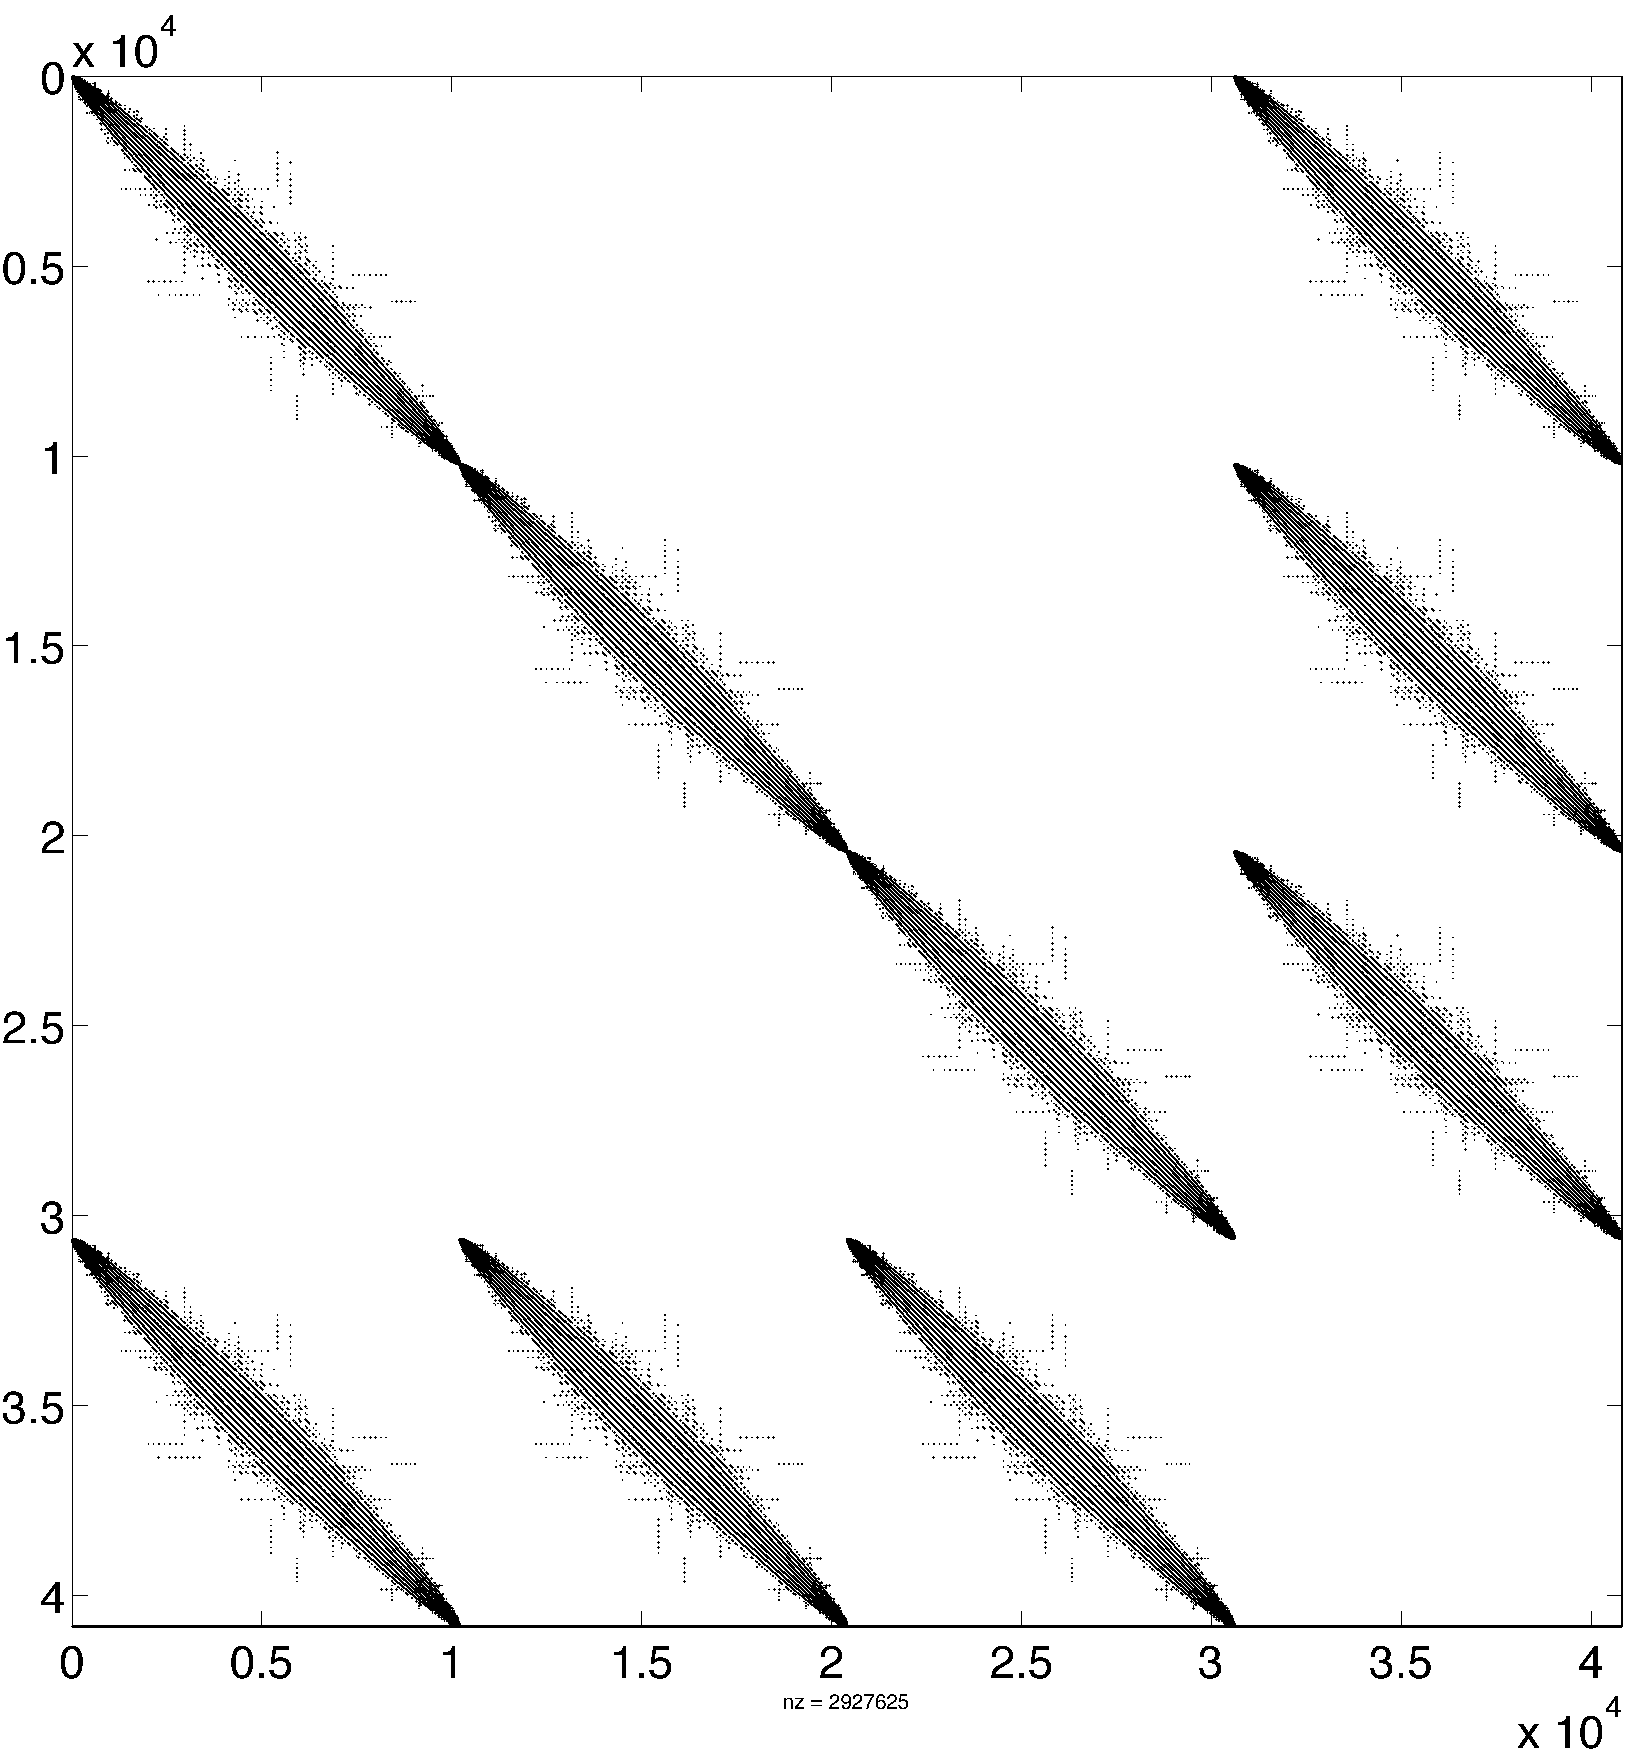
\includegraphics[width=1.0\textwidth]{../figures/paper2/figures/N10201_KDTree_Stokes.pdf} 
		\caption{Grouped by Solution Component}
		\label{fig:original_stokes_dm}
	\end{subfigure}
	\begin{subfigure}[b]{0.4\textwidth}
		\centering
		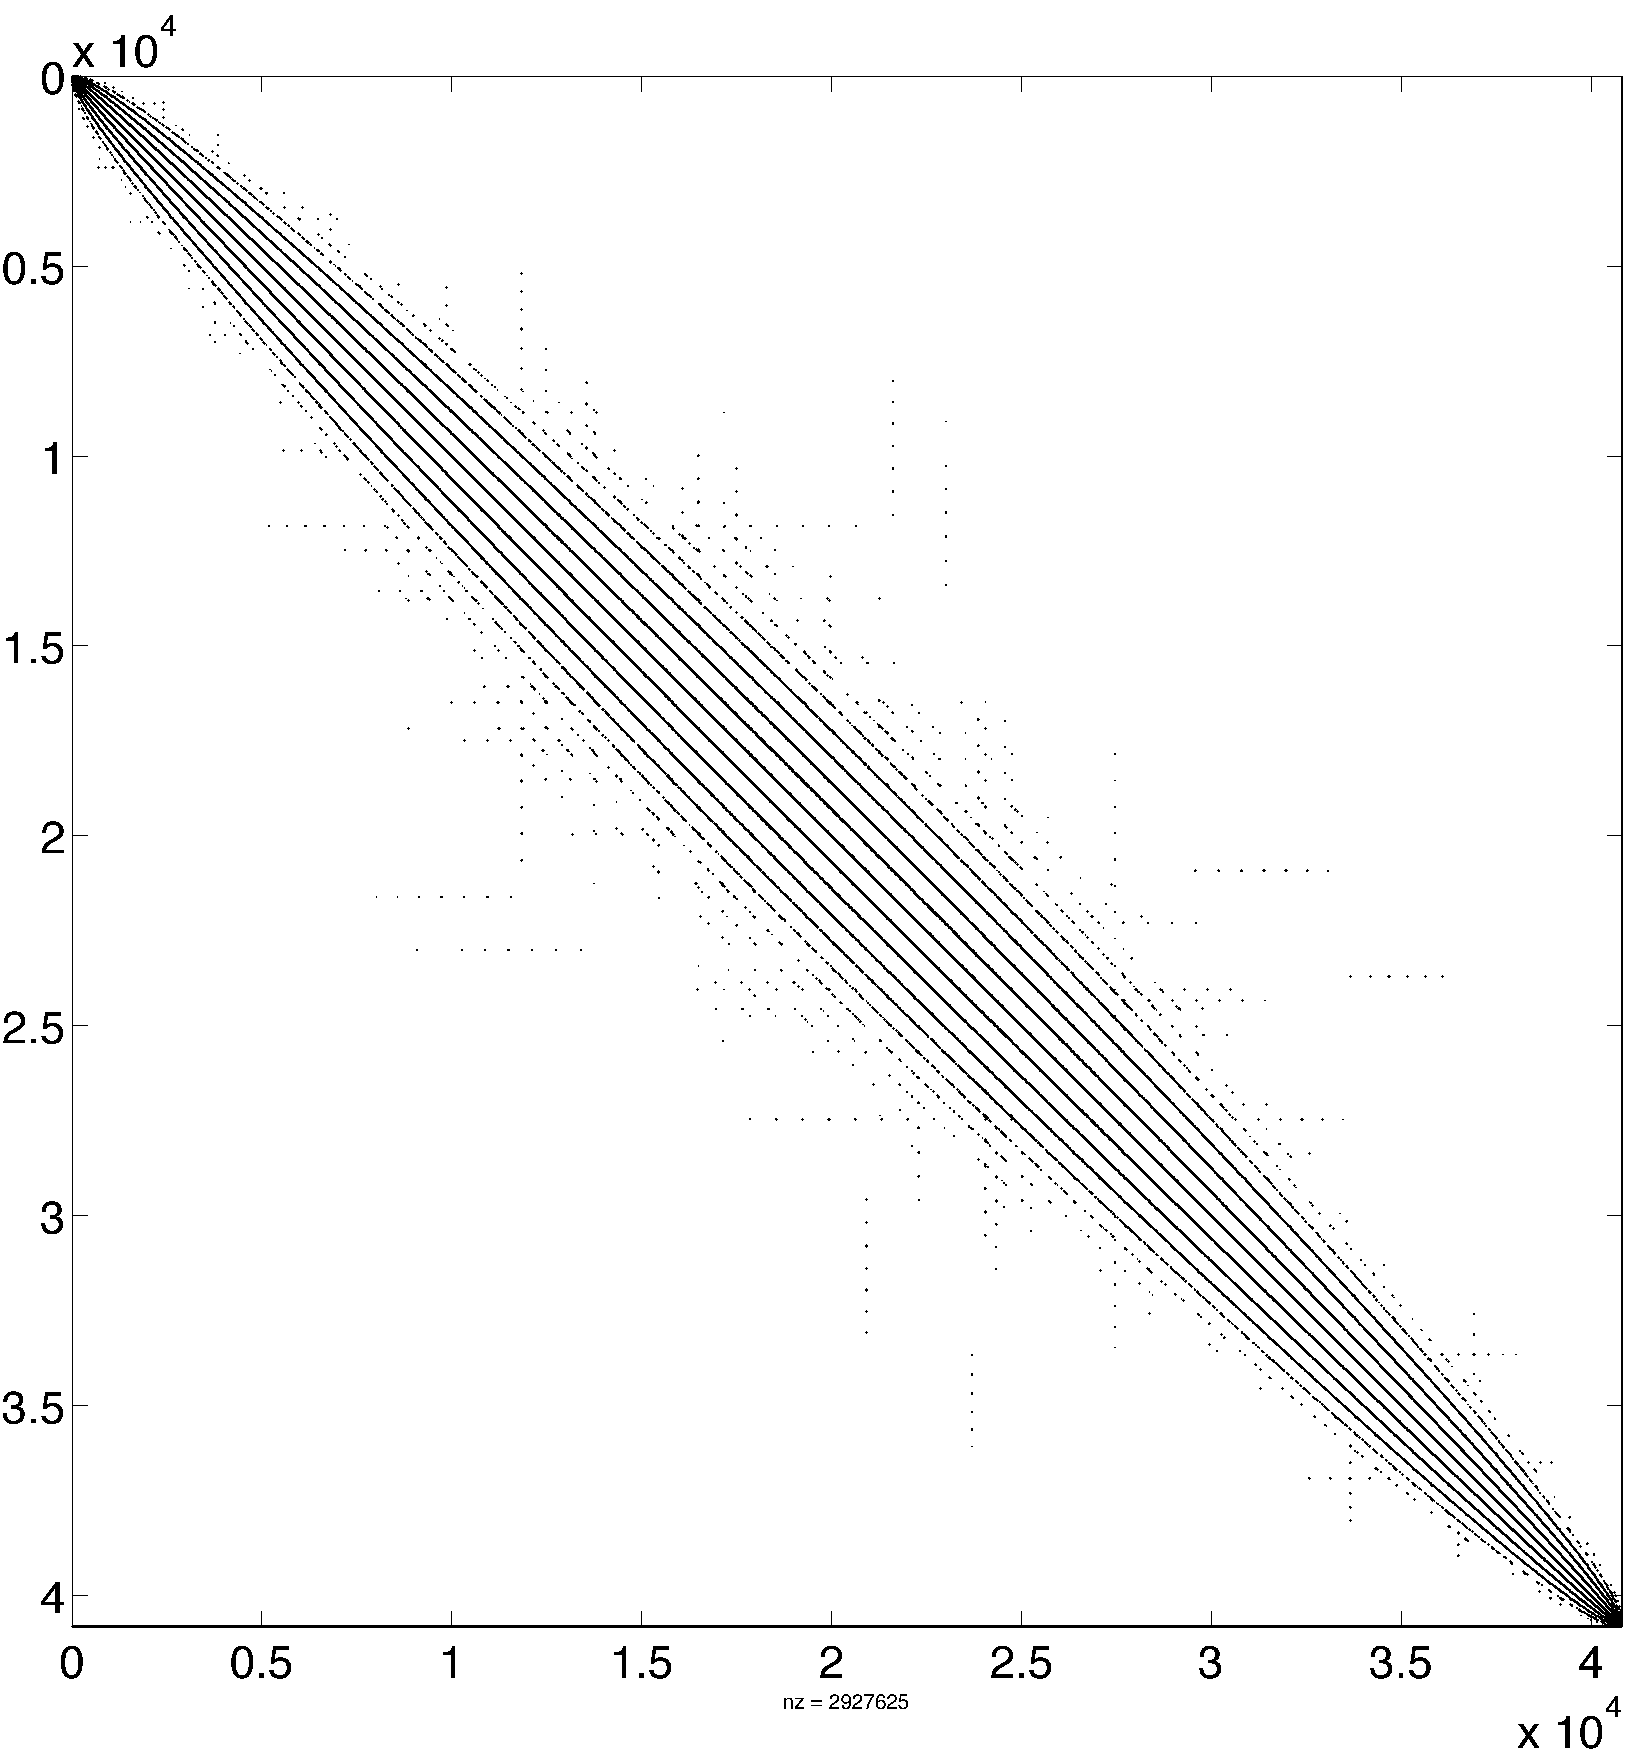
\includegraphics[width=1.0\textwidth]{../figures/paper2/figures/N10201_KDTree_ReorderedStokes.pdf} 
		\caption{Interleaved Solution Components}
		\label{fig:interleaved_stokes_dm}
	\end{subfigure} \\
	\begin{subfigure}[b]{0.4\textwidth}
        		\centering
		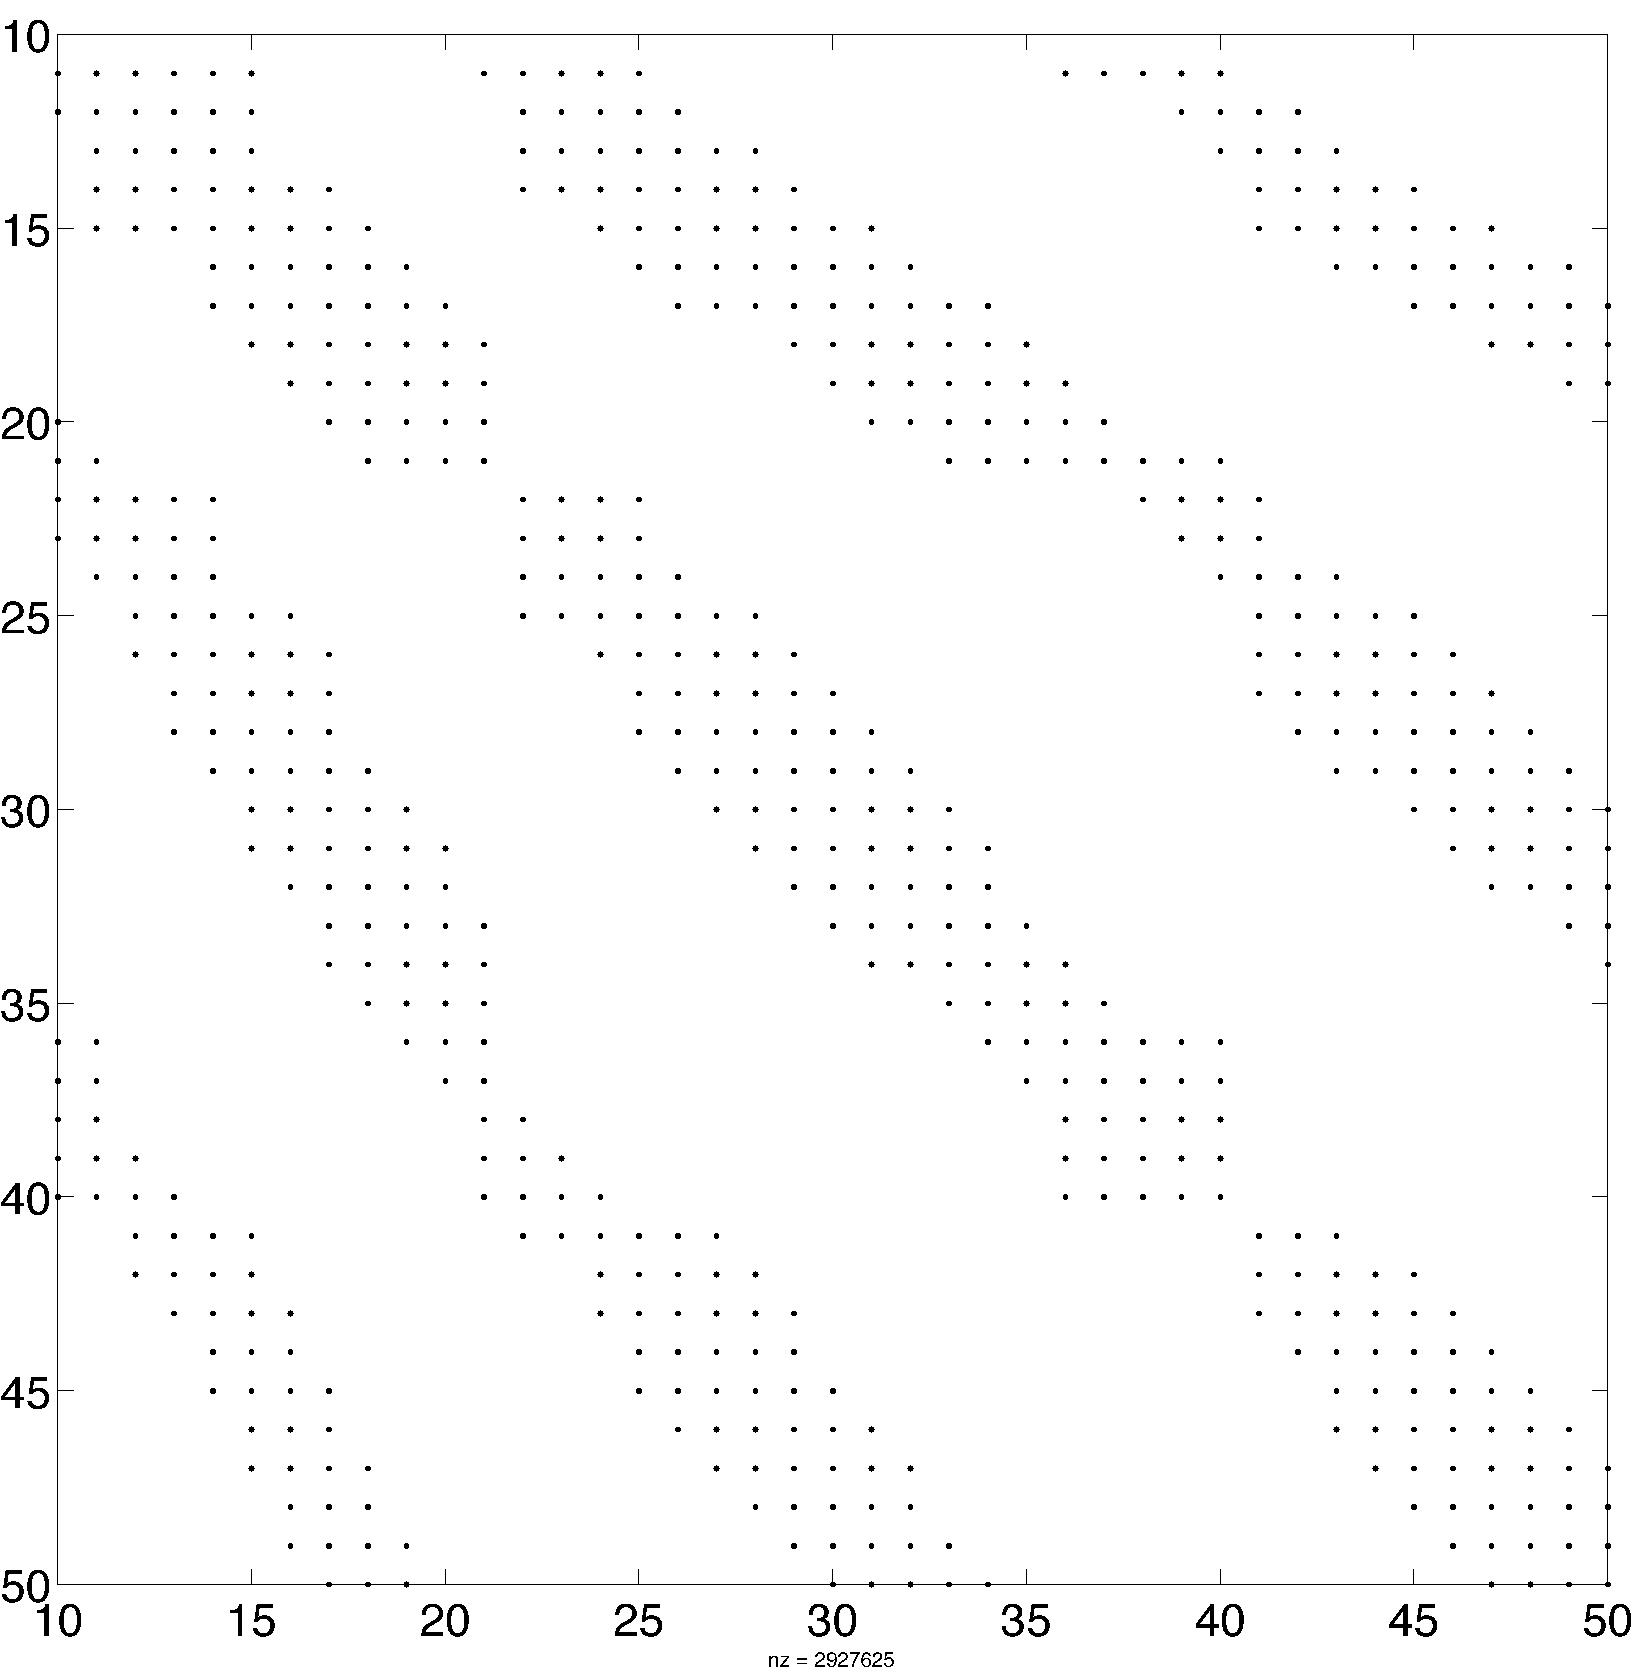
\includegraphics[width=1.0\textwidth]{../figures/paper2/figures/N10201_KDTree_Stokes_10to50.pdf}
		\caption{Grouped Submatrix $(10:50) \times (10:50)$}
		\label{fig:original_stokes_zoom_dm}
	\end{subfigure}
	\begin{subfigure}[b]{0.4\textwidth}
		\centering
	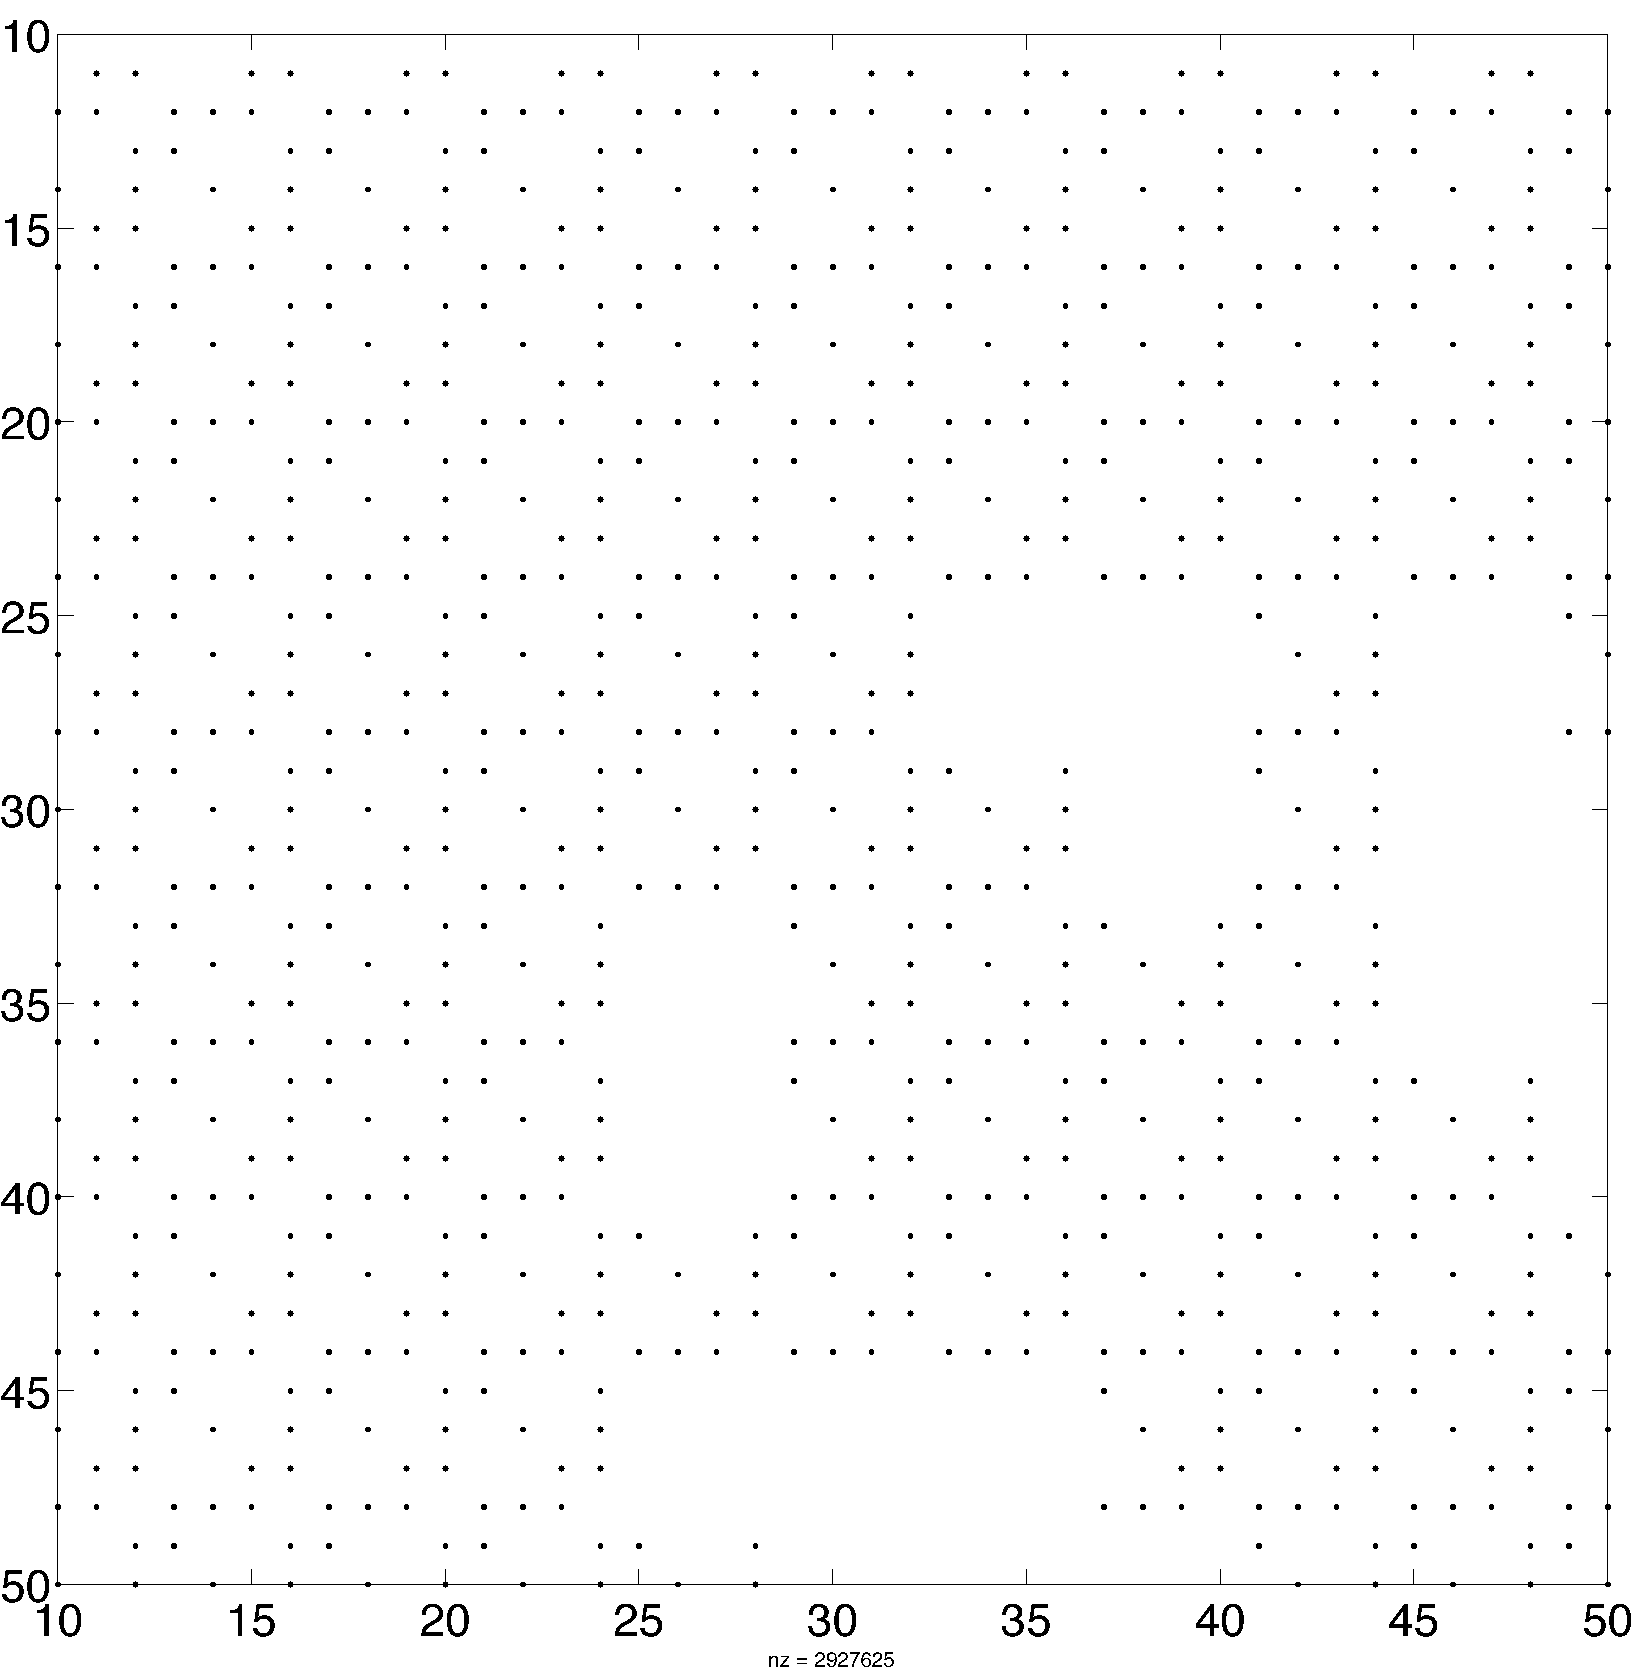
\includegraphics[width=1.0\textwidth]{../figures/paper2/figures/N10201_KDTree_ReorderedStokes_10to50.pdf} 
		\caption{Interleaved Submatrix $(10:50) \times (10:50)$}
		\label{fig:interleaved_stokes_zoom_dm}
	\end{subfigure} \\
\caption{Sparsity pattern of linear system in Equation~\ref{eq:stokes_constant_viscosity}. Solution values are either ordered by component (e.g., $( u_1, \cdots, u_N, v_1, \cdots, v_N, w_1, \cdots, w_N, p_1, \cdots, p_N)^T$) or interleaved (e.g., $( u_1, v_1, w_1, p_1,\cdots, u_N, v_N, w_N, p_N)^T$). }
\label{fig:interleaved_solution}
\end{figure} 


The distributed GMRES implementation depends on two MPI collectives: MPI\_Alltoallv and MPI\_Allreduce. 



We solve the PDE on the surface of the sphere as an example for one and multiple GPUs. 

%TODO: Boundary conditions detract from the accuracy of RBF-FD and introduce other issues such as Runge phenomena \cite{RBFRungePaper}, so we first verify the solution without boundaries. Also, this section 

%TODO: \authnote{ Need to reference work that solves problem in two steps and justify our approach to solve in one step. Golub paper might be good for this. Or the Stoke preconditioners paper. SIMPLE method?  }

Assuming $\eta$ is a constant (i.e., $\grad\eta = 0$), our system simplifies to
\begin{align}
\begin{pmatrix}
-\eta \Laplacian & 0 & 0 & \pd{}{x_1} \\ 
0 & -\eta \Laplacian & 0 & \pd{}{x_2} \\ 
0 & 0 & -\eta \Laplacian & \pd{}{x_3} \\ 
\pd{}{x_1} & \pd{}{x_2} & \pd{}{x_3} & 0 \\
\end{pmatrix} \begin{pmatrix}
u_1 \\ u_2 \\ u_3 \\ p 
\end{pmatrix} = \frac{RaT}{\sqrt{x_1^2 + x_2^2 + x_3^2}}\begin{pmatrix} x_1 \\ x_2 \\ x_3 \\ 0\end{pmatrix}.
\label{eq:stokes_constant_viscosity}
\end{align}
where the $\Laplacian$ operator in spherical polar coordinates for $\mathbb{R}^3$ is: 
\begin{align} 
\Laplacian = \underbrace{\frac{1}{\hat{r}} \pd{}{\hat{r}} \left( \hat{r}^{2} \pd{}{\hat{r}}  \right)}_{\mathsf{radial}} + \underbrace{\frac{1}{\hat{r}^2} \Delta_{S}}_{\mathsf{angular}}.
\end{align}
Here $\LaplaceBeltrami$ is the Laplace-Beltrami operator---i.e., the Laplacian constrained to the surface of the sphere with radius $\hat{r}$. This form nicely illustrates the components of the $\Laplacian$ corresonding to the radial and angular terms. 

On the surface of the unit sphere the radial term vanishes, so we are left with:
\begin{align}
\Laplacian    \equiv \LaplaceBeltrami . 
\end{align}
The following RBF operator from \cite{WrightFlyerYuen10}---Equation (20) can be applied to the RHS of Equation~\ref{eq:rbffd_weight_system} to generate Laplace-Beltrami RBF-FD weights: 
\begin{align} 
\LaplaceBeltrami = \frac{1}{4} \left[ \left(4-r^2\right) \pdd{}{r} + \frac{4-3r^2}{r} \pd{}{r} \right],
\end{align} 
where $r$ is the Euclidean distance between nodes of an RBF-FD stencil and is independent of our choice of coordinate system. 


Additionally following \cite{FlyerWright09, FlyerLehto11}, the off-diagonal blocks in Equation~\ref{eq:stokes_constant_viscosity} must be constrained to the sphere via the projection matrix: 
%\frac{1}{||\mathbf{x}||}
\begin{align}
P = I - \mathbf{x} \mathbf{x}^T =  \begin{pmatrix} 
(1-x_1^2) & -x_1 x_2 & -x_1 x_3 \\
-x_1 x_2 & (1-x_2^2) & -x_2 x_3 \\ 
-x_1 x_3 & -x_2 x_3 & (1-x_3^2) 
\end{pmatrix} = \begin{pmatrix} P_{x_1} \\ P_{x_2} \\ P_{x_3} \end{pmatrix}
\label{eq:gradient_projection}
\end{align}
where $\mathbf{x}$ is the unit normal at the stencil center, and 
%
%Using the chain rule, and assumption that $r(\vx_k-\vx)=\vectornorm{\vx_k-\vx} = \sqrt{(x_{1,k}-x_1)^2 + (x_{2,k}-x_2)^2 + (x_{3,k}-x_3)^2}$, we obtain the unprojected gradient of $\phi$ as
%$$\nabla \phi(r(\vx_k - \vx)) = \pd{r}{\vx} \pd{\phi(r(\vx_k - \vx))}{r} = - (\vx_k - \vx)\frac{1}{r(\vx_k - \vx)} \pd{\phi(r(\vx_k - \vx))}{r}$$. 
%
%Applying the projection matrix gives 
%\begin{align}
%\mathbf{P} \nabla \phi(r(\vx_k - \vx)) & = - (\mathbf{P} \cdot \vx_k - \mathbf{P}\cdot\vx)\frac{1}{r(\vx_k - \vx)} \pd{\phi(r(\vx_k - \vx))}{r} =  - (\mathbf{P}\cdot\vx_k - 0)\frac{1}{r(\vx_k - \vx)} \pd{\phi(r(\vx_k - \vx))}{r} \\
%& = - (I-\vx\vx^T)(\vx_k
%)\frac{1}{r(\vx_k - \vx)} \pd{\phi(r(\vx_k - \vx))}{r} \\
%& = \begin{pmatrix} x \vx^T \vx_k - x_k \\ y \vx^T \vx_k -  y_k \\ z \vx^T \vx_k -z_k \end{pmatrix} \frac{1}{r(\vx_k - \vx)} \pd{\phi(r(\vx_k - \vx))}{r} 
% \end{align}
\cite{FlyerWright09, FlyerLehto11} show that with a little manipulation weights can be directly computed with these operators for Equation~\ref{eq:rbffd_weight_system}: 
%\begin{align} 
%P\pd{}{x_1} = ( x_1 \vx^T \vx_k - x_{1,k}) \frac{1}{d(\vx_k - \vx)} \pd{\phi(d(\vx_k - \vx))}{d} |_{\vx=\vx_j} \\
%P\pd{}{x_2} = ( x_2 \vx^T \vx_k - x_{2,k}) \frac{1}{d(\vx_k - \vx)} \pd{\phi(d(\vx_k - \vx))}{d} |_{\vx=\vx_j} \\
%P\pd{}{x_3} = ( x_3 \vx^T \vx_k - x_{3,k}) \frac{1}{d(\vx_k - \vx)} \pd{\phi(d(\vx_k - \vx))}{d} |_{\vx=\vx_j}
%\end{align}
\begin{align} 
P\pd{}{x_1} = ( x_1 \vx^T \vx_k - x_{1,k}) \frac{1}{r} \pd{}{r} |_{\vx=\vx_j} \\
P\pd{}{x_2} = ( x_2 \vx^T \vx_k - x_{2,k}) \frac{1}{r} \pd{}{r} |_{\vx=\vx_j} \\
P\pd{}{x_3} = ( x_3 \vx^T \vx_k - x_{3,k}) \frac{1}{r} \pd{}{r} |_{\vx=\vx_j}
\end{align}


\subsection{Constraints} 
Due to the lack of boundary conditions on the sphere, the family of solutions that satisfy the PDE in Equation~\ref{eq:stokes_constant_viscosity} includes four free constants (one for each $u_1$, $u_2$, $u_3$ and $p$). 
%In light of this, Equations~\ref{eq:stokes_linear_system} and \ref{eq:stokes_constant_viscosity} are singular with a four-vector null space corresponding to each for the four components of the solution $\begin{pmatrix} u_1, u_2, u_3, p \end{pmatrix}$. 

%The null space is found using the matlab sparse SVD command: \begin{mcode}{1}
%[Usvd, Ssvd, Vsvd, flagSVD] = svds(LHS,10,0);
%sing_value_indices = find(max(Ssvd) < 1e-6)
%\end{mcode} 

%TODO: null-space *of the solution*? or null-space of the equation?
One way to close the null-space of the solution is to augment Equation~\ref{eq:stokes_constant_viscosity} with the following constraints: 
\begin{multline}
\left(\begin{array}{cccc:cccc}  
-\eta \Laplacian & 0 & 0 & \pd{}{x_1} & 1_{N \times 1} & 0 & 0 & 0 \\ 
0 & -\eta \Laplacian & 0 & \pd{}{x_2} & 0 & 1_{N \times 1} & 0 & 0\\ 
0 & 0 & -\eta \Laplacian & \pd{}{x_3} & 0 & 0 & 1_{N \times 1} & 0\\ 
\pd{}{x_1} & \pd{}{x_2} & \pd{}{x_3} & 0 & 0 & 0 & 0 & 1_{N \times 1}\\
\hdashline
1_{1 \times N} & 0 & 0 & 0 & \multicolumn{4}{c}{\multirow{4}{*}{$0_{4 \times 4}$}} \\
0 & 1_{1 \times N} & 0 & 0 & \\
0 & 0 & 1_{1 \times N} & 0 & \\ 
0 & 0 & 0 & 1_{1 \times N} & \\
\end{array} \right) \left(\begin{array}{c} 
u_1 \\ u_2 \\ u_3 \\ p \\ \hdashline c_1 \\ c_2 \\ c_3 \\ c_4
\end{array} \right) \\
 = \frac{RaT}{\sqrt{x_1^2 + x_2^2 + x_3^2}}\begin{pmatrix} x_1 \\ x_2 \\ x_3 \\ 0 \\ \hdashline \int_\Omega u_1 \partial\Omega \\ \int_\Omega u_2 \partial\Omega \\ \int_\Omega u_3 \partial\Omega \\ \int_\Omega p \partial\Omega \end{pmatrix}.
\label{eq:stokes_system_with_constraints}
\end{multline}
%TODO explain this in text: \authnote{Need the integral of my manufactured solution on the RHS. $\ell_1$ norm does not converge to 0, so it will screw solve with constraints}
where the subscript on $1_{N \times 1}$ indicates a $N \times 1$ vector of ones. These constraints add the unknowns $(c_1, c_2, c_3, c_4)$, which should solve to be zero. The four rows on the bottom require that the solution satisfy the integral over the domain for each solution component. In combination with the four added columns, the constraints indicate that the solution components must satisfy integrals using the same constant value. This is only possible if the constants are zero. The added constraints are not physically significant, but are chosen to satisfy the system algebraicly. Of course when solving Equation~\ref{eq:stokes_system_with_constraints} with GMRES, the constraints help increase the rate of convergence. 

%TODO: data to show? 
We also investigate the use of GMRES without constraints. This increases the number of iterations required to converge, but allows increased parallelism (decreased data sharing). %TODO: why is dropping the constraints valid? GMRES assumes zero for each of those? 
%\authnote{Perhaps we can iterate without constraints until convergence slows then ``restart" the problem on a single GPU with constraints included? Limits scalability but would allow more parallelism for part of iterations while also reasonable convergence.}

\subsection{Manufactured Solution}

To verify our implementation, we manufacture a solution that satisfies the continuity equation. Using the identity
\begin{align} 
\div (\curl g(\vx)) = 0,
\end{align} 
for any function $g(\vx)$, we can easily manufacture a solution by choosing some vector function $g(\vx)$, projecting it onto the sphere via $P_x g(x)$ and applying the curl projection, $Q_x$: 
\begin{align} 
Q_x = \begin{bmatrix} 0 & -x_3 & x_2 \\ x_3 & 0 & -x_1 \\ -x_2 & x_1 & 0 \end{bmatrix}.
\end{align} 
Then, a manufactured solution that satisfies both momentum and continuity conditions on the surface of the sphere is given by: 
\begin{align} 
\vu = Q_x (g(\vx))
\end{align} 

Typically, on the surface of the sphere, the projection operator from Equation~\ref{eq:gradient_projection} must be applied to an arbitrary $g(\vx)$. 
Here, we choose the components of $g(\vx)$ to be various spherical harmonics in Cartesian coordinates. Spherical harmonics nicely satisfy $P_x Y_l^m = Y_l^m$. Consequently, the entire application of $P_x$ is neglected. 

%TODO: figure showing spherical harmonics 


We select $g(x)$ to be: 
\begin{align}
g(x) = 8 Y_{3}^{2} - 3Y_{10}^{5} + Y_{20}^{20} 
\end{align}
and the pressure function:
\begin{align}
P = Y_6^4 
\end{align} 

The manufactured solution is shown in Figure~\ref{fig:manufactured_solution}. A Mollweide projection given as: 
\begin{align*}
x &= \frac{2\sqrt{2}}{\pi} \lambda \cos{\theta} \\
y &= \sqrt{2}\sin{\theta}
\end{align*}

 maps the sphere onto the plane. 

\begin{figure} 
\centering
\begin{subfigure}[b]{\textwidth}
\centering
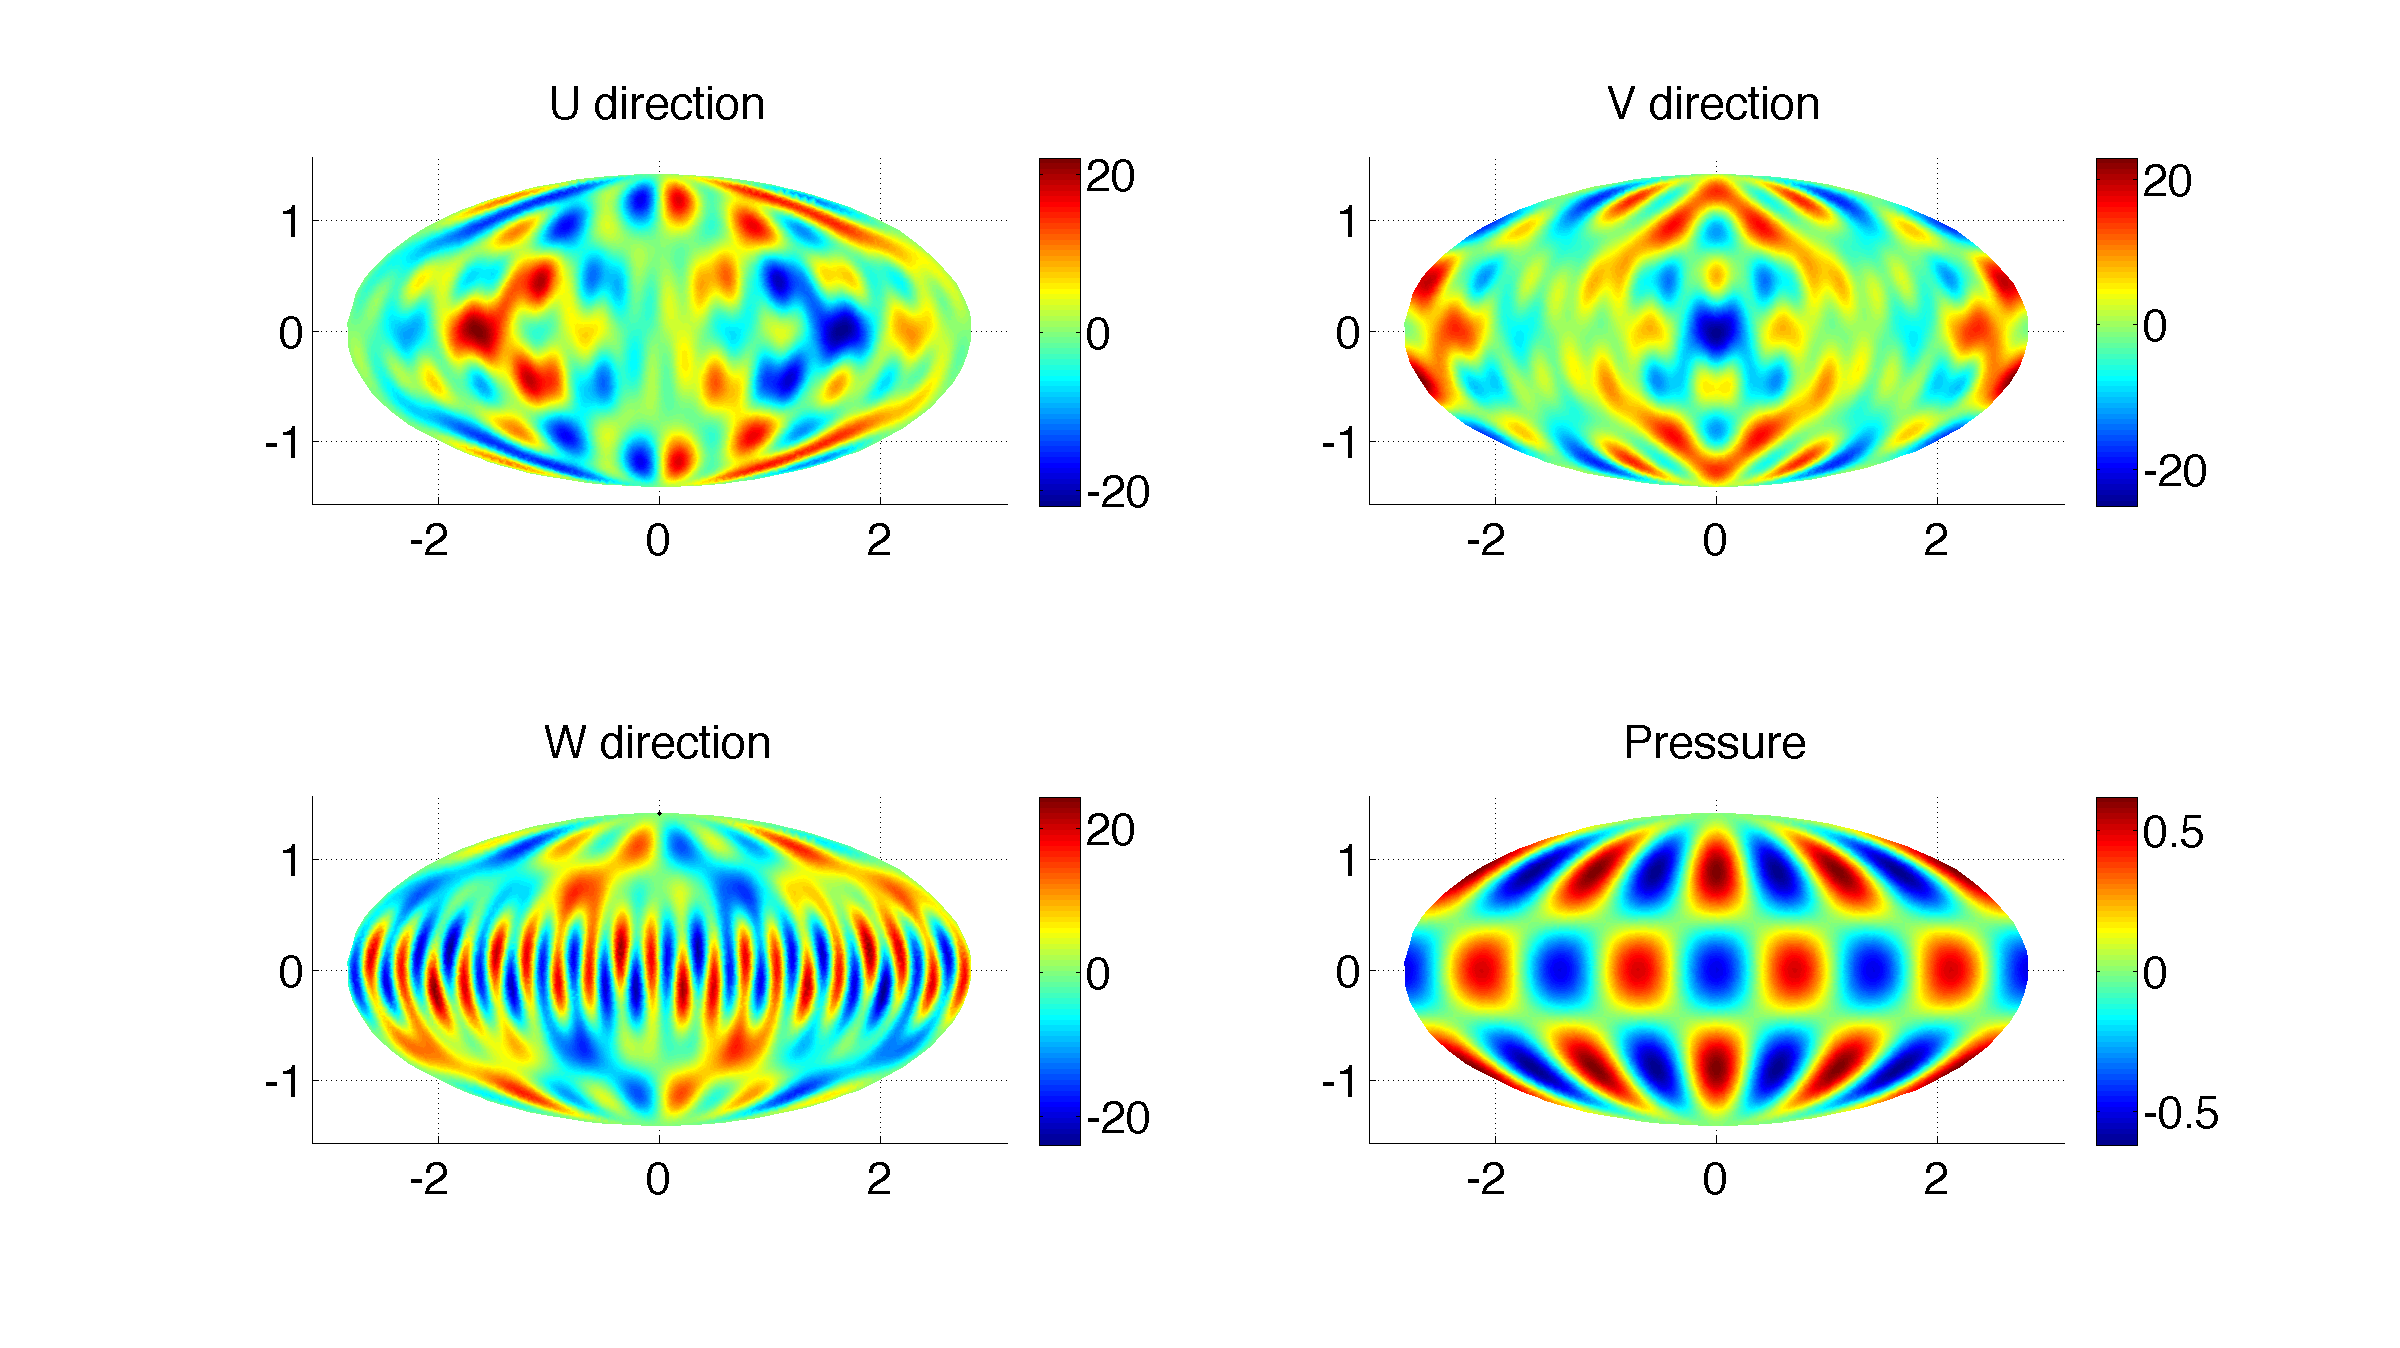
\includegraphics[width=1.0\textwidth]{../figures/paper2/figures/U_exact.png}
\caption{Solution $Q_x( g(x) )$ with $g(x) = 8 Y_{3}^{2} - 3Y_{10}^{5} + Y_{20}^{20}$}
\end{subfigure}
\begin{subfigure}[b]{\textwidth}
\centering
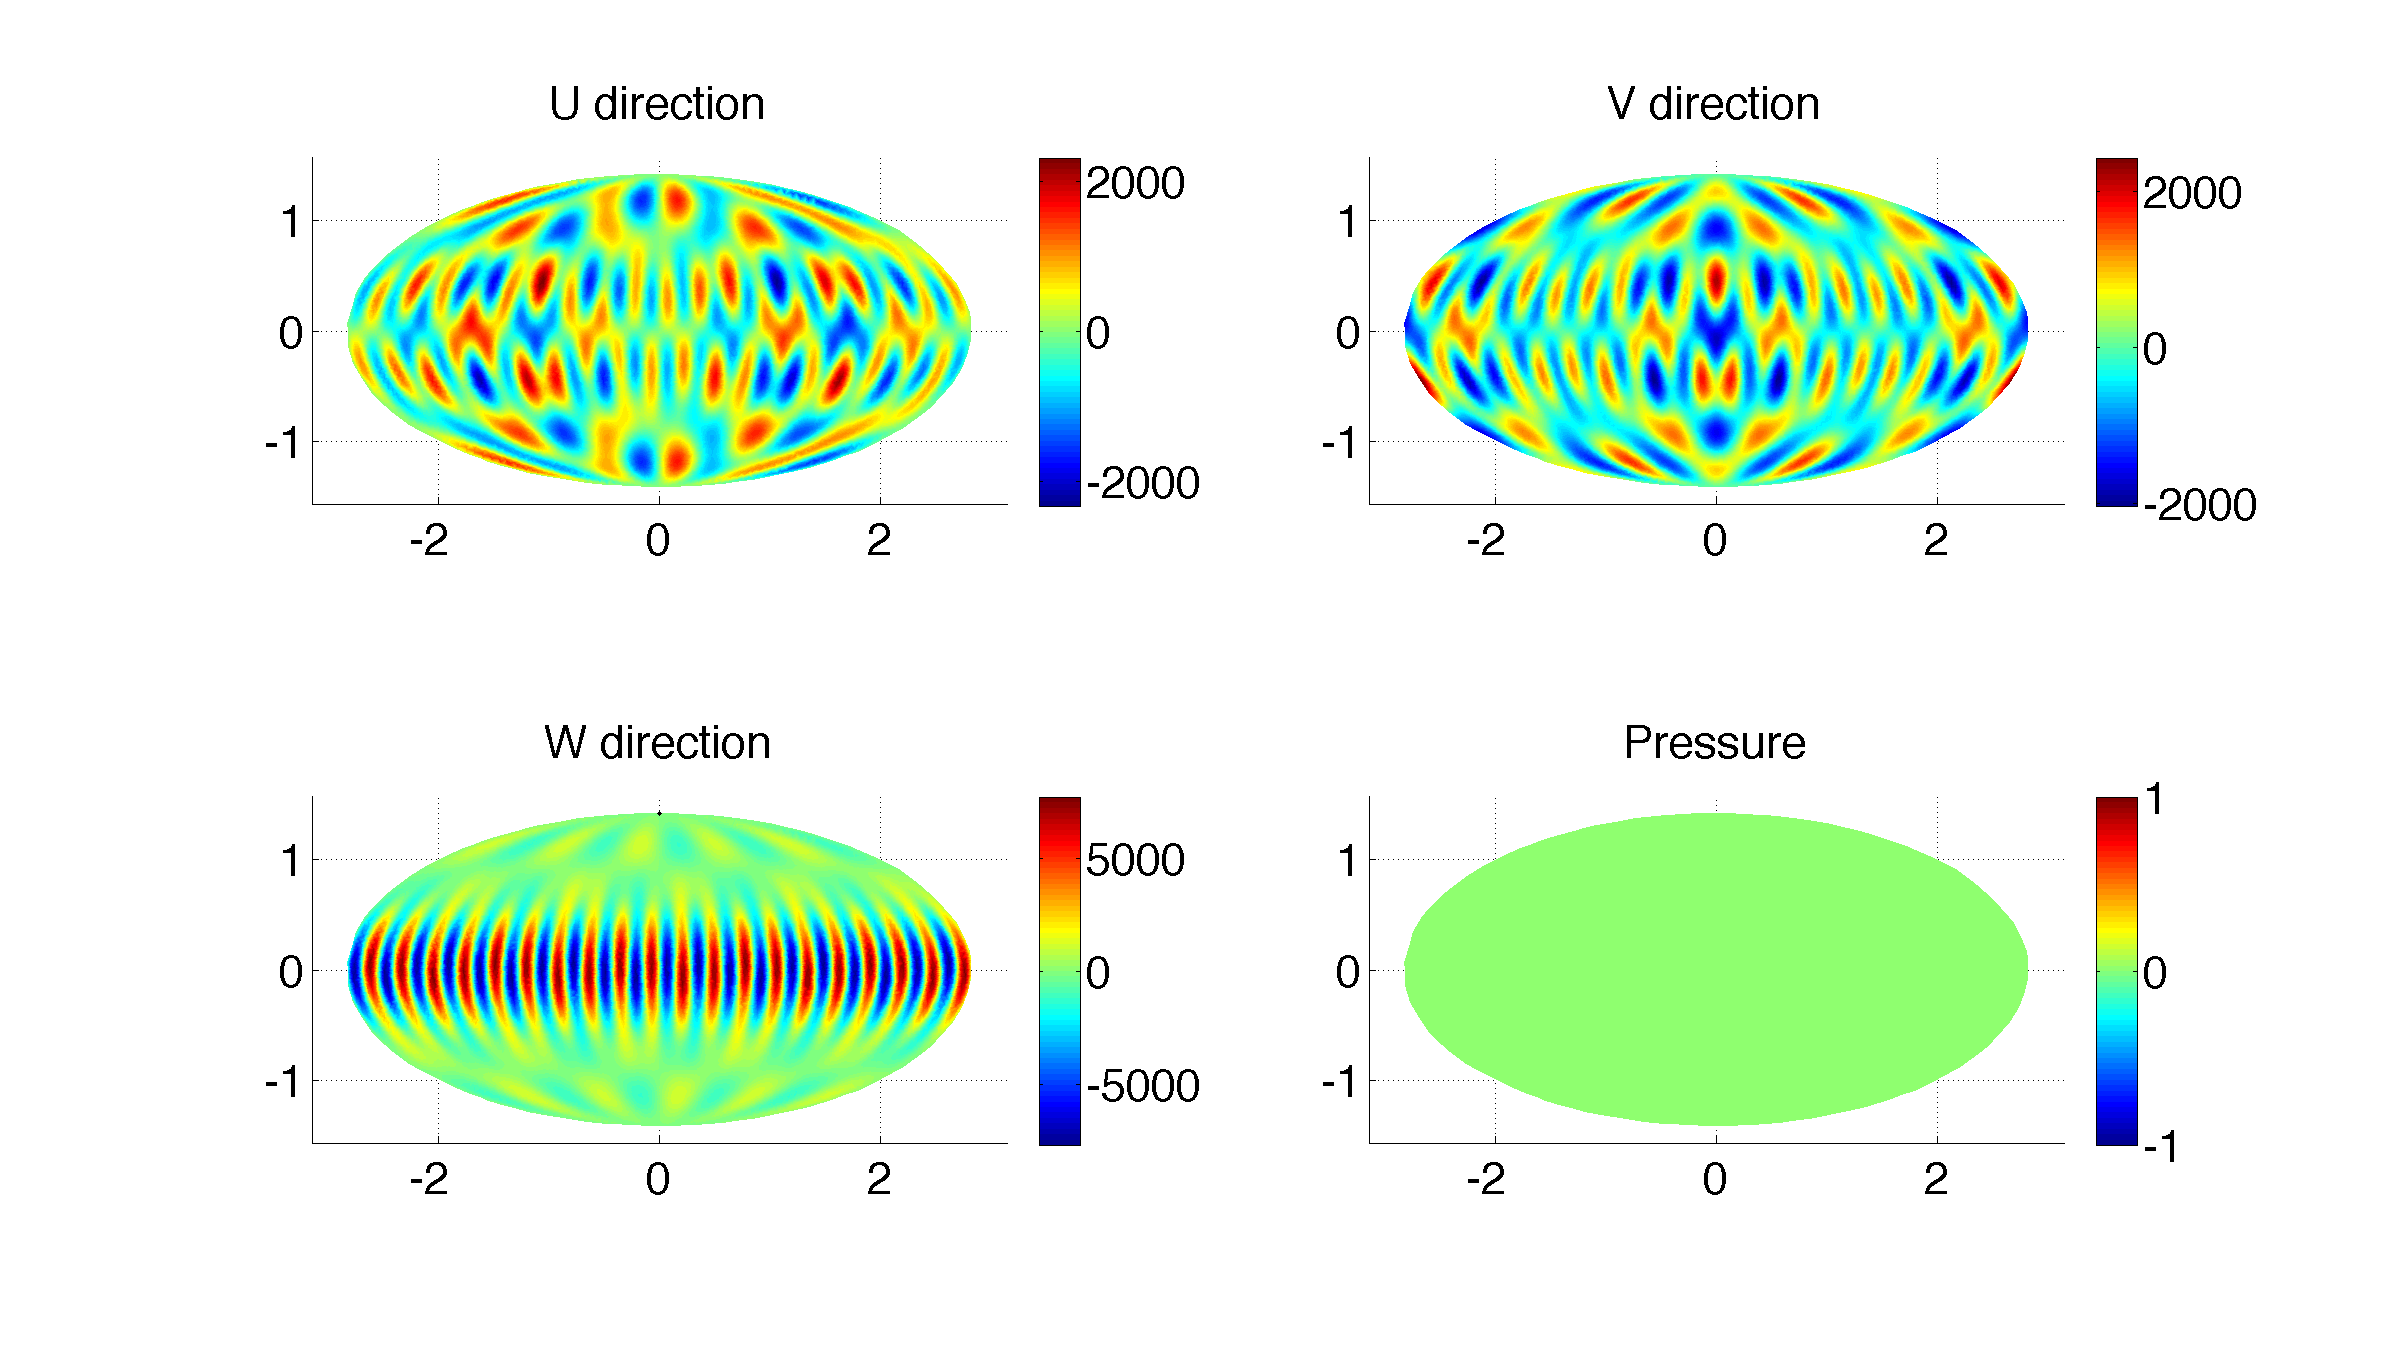
\includegraphics[width=1.0\textwidth]{../figures/paper2/figures/RHS.png}
\caption{Right Hand Side (Constant Viscosity)}
\end{subfigure}
\caption{A divergence free field is manufactured for the sphere. }
\label{fig:manufactured_solution}
\end{figure} 

\subsubsection{Convergence}

%TODO: convergence for Stokes
As the problem size $N$ increases, we expect the approximation to the solution to converge on the order of $\sqrt{n}$ where $n$ is the choice of stencil size. %Figure~\ref{fig:convergence} demonstrates the convergence of our solution with respect to $\sqrt{N}$ for stencil sizes $n=31$, $101$ 

\authnote{Finish convergence plot}. 




\section{Preconditioning} 

GMRES is slow to converge when used without a preconditioner. 

The differentation matrix produced by RBF-FD is asymmetric, non-positive definite, and non-diagonally dominant. Thus, many of the popular choices for preconditioning provided by CUSP and ViennaCL do not apply. 

Our tests show that an incomplete LU factorization with zero fill-in \cite{Saad2003} functions well. 

We also find that a large Krylov subspace must be saved. GMRES converges best when approximately 250 dimensions are saved between restarts. 

%TODO: Plot comparing residual of GMRES without precond and with ILU0 

%TODO:  Need to comment on the conditioning of the system and how stencils can influence convergence


%\authnote{So my matlab code also demonstrates the behavior I was seeing in C++. The $n=31$ case converges VERY quickly with ILU0. However $n=40$ is slow. Another case that works well is $n=110$. I will have to go back and figure out how Im generating the stencils differently. I wonder if the $log(\kappa) = 14$ for $n=40$ is pushing conditioning too high to use? }

%TODO: demonstrate that ILU improve convergence rate (table showing 3 resolutions and convergence with and without ILU)

%TODO: add ILU algorithm
%\begin{algorithm}                     
%\caption{Incomplete LU Factorization with Zero Fill-in (ILU0)}         
%\label{alg:ilu0}                        
%\begin{algorithmic}[1]                  
%    \For i = 0
%    \State $a_{i,i} = a_{i,i} / a_{i,i}$
%    \EndFor
%\end{algorithmic}
%\end{algorithm}

\section{GMRES Results}
%TODO: generate results today

%We want to express benchmarks in terms of the number of GMRES iterations per second, and the number of iterations required to converge. Readers wont 
%care what percentage of peak we are getting, just how fast we get to the solution. 


%\begin{itemize} 
%\item One GPU
%\begin{itemize} 
%	\item {\color{blue} Convergence for stokes steady}  
%	\item {\color{blue} GMRES iteration plot (assuming 1e-8 and restart=60)} 
%\end{itemize} 
%\item Multi-GPU
%	\begin{itemize} 
%		\item Number of iterations without constraints
%		\item Number of iterations with constraints
%		\item GMRES iteration plot
%		\item plot: number of GMRES iterations per second w.r.t. number of processors
%	\end{itemize} 
%\end{itemize} 
%

%
%TODO: State that the conditions under which a problem is solved determines how quickly it will converge. For example, nodes too close together on delaunay meshes cause higher condition numbers and require more iterations. Proper choice of preconditioners can dramatically reduce the number of iterations required to converge. Although preconditioners incur an additional cost in preprocessing and at each iteration of the solver, the potential number of iterations they save 


%John Dennis dissertation has a list of nice datasets (compare the list to Hoth) and their preconditioners. We might list similar paramters used for results here. 
